\chapter[Murmurations: Root Numbers in Frobenius Data]{Murmurations:\\ Root Numbers in Frobenius Data}\label{ch:05b}

For a single elliptic curve the traces of Frobenius forget the root number. They are equidistributed with respect to the Sato Tate law, and the only trace of the sign of the functional equation in a long run of $a_p$ is the slow drift of the rank bias of Section~\ref{sec:05bias}, of size $\log x$ against fluctuations of the same order. In 2022 He, Lee, Oliver and Pozdnyakov \cite{hlop2022} found that this changes completely when one averages over a family at the right scale. Take all curves with conductor in a window $[X,2X)$, average $a_p$ separately over those with root number $+1$ and $-1$, and plot the two averages against $p$: they are mirror images of each other, and both oscillate with a period proportional to the conductor. Plotted against $y=p/N$ the oscillation does not depend on $X$. The shapes were named murmurations, after the flight of starlings, and within two years Zubrilina \cite{zubrilina2023} had proved the analogous statement for modular forms of weight two.

The phenomenon belongs in this book for three reasons. It is a statistic that Proposition~\ref{prop:01limits} does not forbid: it uses for each curve only the finitely many traces at $p\le yN$, and it couples them with an automorphic invariant, the root number, so it is a statement about the family and not about one sequence. It was found by a statistical learning procedure applied to Frobenius data, which is the subject of Chapter~\ref{ch:05}. And it is, as we show in Section~\ref{sec:05bbayes}, a Bayesian identification problem of the kind treated in Chapter~\ref{ch:12}: from about $N/\log N$ traces of a curve one can recover its root number with high probability, and a simple model predicts the error rate.

The chapter is organised as follows. Section~\ref{sec:05bdisc} describes the discovery. Section~\ref{sec:05bdef} gives the definition and explains, through the trace formula, why the natural scale is $p/N$. Section~\ref{sec:05blit} states what has been proved. Section~\ref{sec:05bdata} reports our computation for all $30{,}366$ isogeny classes of conductor between $2500$ and $10000$, and Section~\ref{sec:05brank} separates the ranks. Section~\ref{sec:05bbayes} treats the recovery of root numbers as Bayesian classification, and Section~\ref{sec:05bthorin} places murmurations against the one level density of Chapter~\ref{ch:06} and the Thorin measures of Chapter~\ref{ch:10b}, and Section~\ref{sec:05bram} traces the tools back to Ramanujan and Mordell and computes murmurations in Ramanujan's family of level one forms.

\section{The discovery}\label{sec:05bdisc}

He, Lee, Oliver and Pozdnyakov trained standard classifiers (logistic regression, naive Bayes, small neural networks) to predict the rank of an elliptic curve over $\Q$ from the vector $(a_2,a_3,a_5,\dots,a_p)$ of its first few hundred traces, using the curves in the LMFDB \cite{lmfdb}. The classifiers did far better than chance at separating rank $0$ from rank $1$. That in itself is not surprising, since the rank bias of Section~\ref{sec:05bias} already makes $\sum_p a_p\log p/p$ informative about the rank. What was surprising came from inspecting what the classifiers had learned: averaging $a_p$ over all curves of rank $0$ with conductor in a fixed range, and separately over the curves of rank $1$, produced two curves in $p$ that oscillated in opposite phase with a period of order the conductor. Rank enters only through its parity, that is through the root number $\varepsilon_E=(-1)^{r_E}$, and the effect is a property of the family, invisible for any single curve.

Sarnak, in a letter to Sutherland and Zubrilina \cite{sarnakletter2023}, explained the phenomenon for modular forms through the Eichler Selberg trace formula and posed the problem of proving it. Zubrilina did so in the conductor aspect \cite{zubrilina2023}, and the method was quickly carried to other families: modular forms in the weight aspect by Bober, Booker, Lee and Lowry Duda \cite{bbllp2023}, and Dirichlet characters by Lee, Oliver and Pozdnyakov \cite{lop2023}. For elliptic curves themselves, ordered by conductor, no proof is known. Sawin and Sutherland \cite{sawinsutherland2025} treated curves ordered by naive height, proving a theorem for a smoothed variant of the average and formulating a conjecture for the murmuration density as a sum of Bessel functions.

\section{Definition and scale}\label{sec:05bdef}

\begin{definition}\label{def:05bmurm}
Let $\mathcal{F}_X$ be the set of isogeny classes of elliptic curves over $\Q$ with conductor $N_E\in[X,2X)$, represented by one curve $E$ each. For $E\in\mathcal{F}_X$ write $a_p(E)=p+1-\#E(\mathbb{F}_p)$ for $p\nmid N_E$ and let $a_p(E)\in\{0,\pm1\}$ be the usual value at the bad primes, and let $\varepsilon_E\in\{\pm1\}$ be the root number. For $0<y_1<y_2$ the \emph{murmuration average} of $\mathcal{F}_X$ on $[y_1,y_2)$ is
\[
D_X(y_1,y_2)=\frac{\sum_{E\in\mathcal{F}_X}\sum_{p:\,y_1\le p/N_E<y_2}\varepsilon_E\,a_p(E)}{\#\{(E,p):E\in\mathcal{F}_X,\ y_1\le p/N_E<y_2\}},
\]
and, for a bin width $h>0$, the empirical murmuration density is $D_X(y)=D_X(y,y+h)$.\index{murmuration}
\end{definition}

The trace $a_p(E)$ is not normalised by $\sqrt p$. This is deliberate: the average of $\varepsilon_Ea_p(E)$ at $p\asymp yN$ is of order one, so that $D_X(y)$ has a limit in $X$ without rescaling, whereas the average of $\varepsilon_Ea_p(E)/\sqrt p$ decays like $X^{-1/2}$. Our data confirm this (Section~\ref{sec:05bdata}).

Why should the right scale be $p/N$, and why should the average be of order one? For newforms the answer comes from the trace formula. Let $f$ run over the newforms of weight two and trivial character on $\Gamma_0(N)$, with Hecke eigenvalues $a_f(p)$, and let $W_N$ be the Atkin Lehner involution, with eigenvalue $w_f=\pm1$ on $f$. The root number of $L(s,f)$ is $\varepsilon_f=-w_f$. Hence
\[
\sum_f\varepsilon_f\,a_f(p)=-\operatorname{tr}\bigl(T_p\circ W_N\mid S_2^{\mathrm{new}}(N)\bigr),
\]
the trace of the composite of a Hecke operator with the Atkin Lehner involution. Traces of this kind were computed by Yamauchi \cite{yamauchi1973} in the form of an Eichler Selberg trace formula. Its main terms are Hurwitz class numbers of discriminants of the form $t^2N^2-4pN$, summed over the integers $t$ with $t^2N<4p$, that is with $t^2<4y$. The number of terms depends only on $y=p/N$; each class number is of size about $\sqrt{pN}$; and the dimension of $S_2^{\mathrm{new}}(N)$ is of order $N$. So the average of $\varepsilon_fa_f(p)$ over the family is of order $\sqrt{pN}/N=\sqrt y$, a function of $y$ alone, with new terms entering whenever $y$ crosses one of the values $t^2/4$. This is the heuristic that Zubrilina made rigorous. The elliptic curves are the newforms with rational coefficients, a sparse subfamily, and nothing in the trace formula forces them to inherit the density of the full family; that they appear to do so is part of the mystery.

\begin{remark}
In the language of Chapter~\ref{ch:07} the vertical Sato Tate law is the statement that the averages of $a_f(p)/\sqrt p$ over a family converge to the Plancherel measure as $N\to\infty$ with $p$ fixed. Murmurations live at the other end, with $p$ growing in proportion to $N$, where the trace formula no longer reduces to its identity term and the hyperbolic and elliptic terms that carry the class numbers take over. The root number enters because $W_N$ does, and $W_N$ is visible in the trace only when $p$ is comparable to $N$.
\end{remark}

\section{What is proved}\label{sec:05blit}

We state the results in words, since their exact normalisations differ from ours and from one another.

\begin{theorem}[Zubrilina \cite{zubrilina2023}]\label{thm:05bzub}
Let $f$ run over the newforms of weight two and trivial character whose level $N$ is squarefree and lies in $[X,X+cX)$, for a fixed $c>0$. For fixed $0<y_1<y_2$, the average of $\varepsilon_f\,a_f(p)$ over the pairs $(f,p)$ with $y_1\le p/N<y_2$, suitably normalised, converges as $X\to\infty$ to $\int_{y_1}^{y_2}M(y)\,dy$, where $M$ is an explicit continuous function given by the trace formula of Section~\ref{sec:05bdef}.
\end{theorem}

\begin{theorem}[Bober, Booker, Lee and Lowry Duda \cite{bbllp2023}; Lee, Oliver and Pozdnyakov \cite{lop2023}]
The analogue of Theorem~\ref{thm:05bzub} holds for holomorphic newforms of level one in the weight aspect, with the scale $p/k^2$, and for primitive Dirichlet characters ordered by conductor, with the root number replaced by the normalised Gauss sum.
\end{theorem}

For elliptic curves ordered by naive height, Sawin and Sutherland \cite{sawinsutherland2025} prove a theorem for a smoothed version of the average, obtained by summing over integers with no small prime factors and using the Voronoi summation formula, and they conjecture the murmuration density in closed form as a sum of Bessel functions. They tested the conjecture on curves of height up to $2^{28}$, and gave a separate predicted density for curves of prime conductor ordered by conductor. For elliptic curves ordered by conductor, the ordering of He, Lee, Oliver and Pozdnyakov and the one used in this chapter, the existence of a limiting density is open (Open Problem~\ref{op:05bcond}).

\section{The data}\label{sec:05bdata}

We used every isogeny class of conductor $2500\le N<10000$ in Cremona's tables \cite{cremonaecdata}, represented by the first curve of the class, with its analytic rank $r_E$, which for these conductors is known and gives $\varepsilon_E=(-1)^{r_E}$. For each curve we computed $a_p$ for all $p<15000$ in the window $[2500,5000)$ and all $p<30000$ in the window $[5000,10000)$, with \texttt{ellan} in PARI/GP \cite{pari2023}, so that every pair with $p/N\le3$ is present. The two windows contain $9{,}638$ and $20{,}728$ classes; their ranks are distributed as in Table~\ref{tab:05branks}.

\begin{table}[ht]
\centering
\begin{tabular}{lrrrrr}
\toprule
Window & classes & rank $0$ & rank $1$ & rank $2$ & rank $3$ \\
\midrule
$2500\le N<5000$ & $9{,}638$ & $4{,}187$ & $5{,}030$ & $421$ & $0$ \\
$5000\le N<10000$ & $20{,}728$ & $8{,}536$ & $10{,}811$ & $1{,}380$ & $1$ \\
\bottomrule
\end{tabular}
\caption{Isogeny classes in the two conductor windows, by analytic rank.}\label{tab:05branks}
\end{table}

Figure~\ref{fig:05bdensity} shows the result. On the left are the averages of $a_p$ over the classes of root number $+1$ and $-1$ in the window $[5000,10000)$, in $150$ bins of $p$; they are mirror images up to noise, which is murmuration in its original form. On the right is the empirical density $D_X(y)$ for both windows, with bin width $h=0.025$ on $0<y\le3$.

\begin{figure}[ht]
\centering
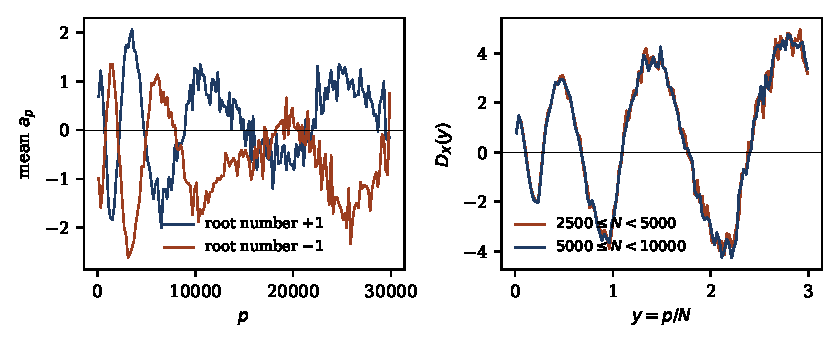
\includegraphics[width=\textwidth]{figs/murm_density.pdf}
\caption{Murmurations of elliptic curves over $\Q$. Left: mean $a_p$ over the isogeny classes with $5000\le N<10000$ and root number $+1$ (blue) and $-1$ (red), in bins of $p$. Right: the empirical murmuration density $D_X(y)$ of Definition~\ref{def:05bmurm}, bin width $0.025$, for the windows $[2500,5000)$ and $[5000,10000)$.}\label{fig:05bdensity}
\end{figure}

Three features stand out.

\begin{enumerate}
\item Scale invariance. The two curves on the right of Figure~\ref{fig:05bdensity} coincide to within noise: their correlation over the $120$ bins is $0.994$ and their root mean squares are $2.736$ and $2.746$. The windows differ by a factor of two in conductor, so a decay like $X^{-1/2}$ would have shown as a ratio of $1.41$; in the normalisation with $a_p/\sqrt p$ in place of $a_p$, that is exactly the ratio we observe ($1.40$ by least squares).
\item Oscillation with growing amplitude. In the window $[5000,10000)$ the density is positive near $y=0$, changes sign near $y=0.11$, $0.29$, $0.69$, $1.11$, $1.79$ and $2.41$, and its extreme values on $(0.3,3]$ are $-4.27$ near $y=2.21$ and $4.75$ near $y=2.79$. The amplitude grows roughly like $\sqrt y$, as the trace formula heuristic of Section~\ref{sec:05bdef} predicts. The largest standard error of a bin is $0.25$.
\item A positive bias. Averaged over all pairs with $p/N\le3$, $\varepsilon_Ea_p(E)/\sqrt p$ has mean $0.0071$ with standard error $0.00014$. The sign is that of the rank bias of Section~\ref{sec:05bias}: the classes of root number $+1$ are mostly of rank $0$, which tilts the traces up, and those of root number $-1$ mostly of rank $1$, which tilts them down.
\end{enumerate}

\section{Root number or rank?}\label{sec:05brank}

The root number is determined by the parity of the rank, but the rank carries more. Figure~\ref{fig:05brank} shows the mean of $a_p$, without the sign $\varepsilon_E$, separately for the classes of rank $0$, $1$ and $2$ in the window $[5000,10000)$. Ranks $0$ and $2$ share the root number $+1$ and follow the same oscillation; rank $1$ is its mirror image. The averages of $a_p/\sqrt p$ over all pairs with $p/N\le3$ are $+0.0079$, $-0.0106$ and $-0.0246$ for ranks $0$, $1$ and $2$. These decrease with the rank, as the drift $\frac12-r$ of Section~\ref{sec:05bias} predicts, while the oscillation follows the parity. So the family average decomposes into two pieces with different origins: an oscillating term at the scale $p\asymp N$ governed by the root number, which the trace formula produces, and a slowly varying bias governed by the rank, which the explicit formula produces. For rank $2$ the two pull in opposite directions, which is why, in the next section, root numbers of rank $2$ curves are the hardest to recover.

\begin{figure}[ht]
\centering
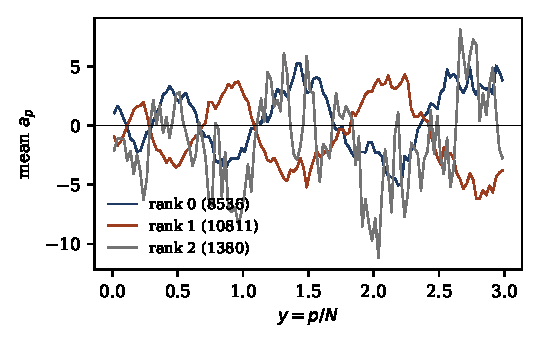
\includegraphics[width=0.62\textwidth]{figs/murm_rank.pdf}
\caption{Mean $a_p$ in bins of $y=p/N$ for the isogeny classes with $5000\le N<10000$ of rank $0$, $1$ and $2$ (numbers of classes in brackets).}\label{fig:05brank}
\end{figure}

\section{Root numbers as Bayesian classification}\label{sec:05bbayes}

\subsection{A model}

Fix a curve $E$ of conductor $N$, a cutoff $y>0$ and the set $P=\{p\le yN\}$. Write $x_p=a_p(E)/\sqrt p\in[-2,2]$. The simplest model in which murmurations carry information about $\varepsilon_E$ is the following.

\begin{definition}\label{def:05bmodel}
Under the \emph{murmuration model} with weights $(m_p)_{p\in P}$, the root number $\varepsilon\in\{\pm1\}$ has prior probability $\frac12$ for each value, and given $\varepsilon$ the $x_p$, $p\in P$, are independent with values in $[-2,2]$ and means $\E[x_p\mid\varepsilon]=\varepsilon m_p$. The \emph{murmuration score} is $S=\sum_{p\in P}m_px_p$, and its \emph{signal} is $V=\sum_{p\in P}m_p^2$.
\end{definition}

The family average of Section~\ref{sec:05bdef} suggests $m_p=D(p/N)/\sqrt p$, with $D$ the limiting density. The model ignores the rank bias and every dependence between the traces of one curve; we test it against the data below.

\begin{proposition}\label{prop:05bclass}
Under the murmuration model:
\begin{enumerate}
\item $\E[\varepsilon S\mid\varepsilon]=V$;
\item the classifier $\hat\varepsilon=\operatorname{sign}S$ errs with probability at most $e^{-V/8}$;
\item if, moreover, $x_p\mid\varepsilon$ is normal with mean $\varepsilon m_p$ and variance $1$ (ignoring the bound $|x_p|\le2$), then the posterior probability is $\Prob(\varepsilon=+1\mid x)=1/(1+e^{-2S})$, $\hat\varepsilon$ is the Bayes rule, and its error probability is exactly $\Phi(-\sqrt V)$, with $\Phi$ the standard normal distribution function.
\end{enumerate}
\end{proposition}

\begin{proof}
(1) By linearity, $\E[\varepsilon S\mid\varepsilon]=\sum_pm_p\,\varepsilon\E[x_p\mid\varepsilon]=\sum_pm_p^2$.
(2) Given $\varepsilon$, $\varepsilon S-V=\sum_pm_p(\varepsilon x_p-m_p)$ is a sum of independent centred terms, the term of $p$ taking values in an interval of length $4|m_p|$. Hoeffding's inequality gives $\Prob(\varepsilon S-V\le-V\mid\varepsilon)\le\exp(-2V^2/\sum_p16m_p^2)=e^{-V/8}$, and an error requires $\varepsilon S\le0$.
(3) The log likelihood ratio is $\sum_p\frac12\bigl[(x_p+m_p)^2-(x_p-m_p)^2\bigr]=2S$, which with equal priors gives the posterior and shows that $\operatorname{sign}S$ maximises it. Given $\varepsilon=+1$, $S$ is normal with mean $V$ and variance $V$, so $\Prob(S\le0)=\Phi(-\sqrt V)$, and symmetrically for $\varepsilon=-1$.
\end{proof}

\begin{lemma}\label{lem:05bsignal}
Let $0<y_0<y$ and let $D$ be continuous and of bounded variation on $[y_0,y]$. Then, as $N\to\infty$,
\[
\sum_{y_0N<p\le yN}\frac{D(p/N)^2}{p}=\frac{1+o(1)}{\log N}\int_{y_0}^{y}\frac{D(t)^2}{t}\,dt.
\]
\end{lemma}

\begin{proof}
Put $g=D^2$, which is continuous and of bounded variation. By partial summation,
\[
\sum_{y_0N<p\le yN}\frac{g(p/N)}{p}=\int_{y_0N}^{yN}\frac{g(x/N)}{x}\,d\pi(x).
\]
Write $\pi(x)=\operatorname{li}(x)+R(x)$ with $R(x)=o(x/\log x)$ by the prime number theorem. The main term is $\int_{y_0N}^{yN}g(x/N)\,dx/(x\log x)=\int_{y_0}^{y}g(t)\,dt/(t\log(Nt))$, which is $(1+O(1/\log N))(\log N)^{-1}\int_{y_0}^yg(t)\,dt/t$. Integrating by parts, the remainder is bounded by $\sup|R(x)/x|$ over $[y_0N,yN]$ times a constant depending on $y_0$, $y$, $\sup|g|$ and the total variation of $g$, and this is $o(1/\log N)$.
\end{proof}

With the weights $m_p=D(p/N)/\sqrt p$ of the family density, the signal $V$ over the primes in $(y_0N,yN]$ is therefore of order $1/\log N$ for fixed $y_0$ and $y$. If the murmuration model were exact and the density did not change with $X$, the power of the score at a fixed cutoff $y$ would decay slowly, like $\Phi(-c/\sqrt{\log N})$ on that range, as the conductor grows; with all $y\le Y$ and $Y$ growing, it would grow. The small primes $p\le y_0N$, where $D$ need not vanish and the rank bias is felt, are what the lemma leaves out.

\subsection{Test against the data}

We split the $20{,}728$ classes of the window $[5000,10000)$ at random into two halves. On the first half we estimated the density of $\varepsilon_Ea_p(E)/\sqrt p$ in bins of $y$ of width $0.025$; this is $m_p$ of Definition~\ref{def:05bmodel} up to the bin. On the second half, and on all $9{,}638$ classes of the window $[2500,5000)$, we computed the score $S_E$ with the primes $p\le yN_E$ for several cutoffs $y$, and predicted $\varepsilon_E=\operatorname{sign}S_E$. Table~\ref{tab:05bclass} gives the results. The commoner root number in the test half has frequency $0.521$, so that is the accuracy of guessing.

\begin{table}[ht]
\centering
\begin{tabular}{rrrrrrr}
\toprule
$y$ & accuracy & transfer & mean $\varepsilon S$ & sd $\varepsilon S$ & $V$ & $\Phi(-\sqrt V)$ \\
\midrule
$0.25$ & $0.865$ & $0.891$ & $0.907$ & $0.843$ & $0.905$ & $0.171$ \\
$0.5$ & $0.896$ & $0.915$ & $1.247$ & $0.998$ & $1.232$ & $0.134$ \\
$1$ & $0.924$ & $0.941$ & $1.671$ & $1.118$ & $1.656$ & $0.099$ \\
$1.5$ & $0.937$ & $0.949$ & $1.992$ & $1.273$ & $1.983$ & $0.080$ \\
$2$ & $0.941$ & $0.952$ & $2.125$ & $1.332$ & $2.119$ & $0.073$ \\
$3$ & $0.952$ & $0.962$ & $2.595$ & $1.521$ & $2.582$ & $0.054$ \\
\bottomrule
\end{tabular}
\caption{Recovery of root numbers from the murmuration score with the primes $p\le yN$. Accuracy: held out half of $5000\le N<10000$. Transfer: all classes with $2500\le N<5000$, scored with the density learned on the other window. The mean and standard deviation of $\varepsilon S$ and the average signal $V$ refer to the held out half; the last column is the error predicted by Proposition~\ref{prop:05bclass}(3).}\label{tab:05bclass}
\end{table}

The model passes two of its three checks. Part (1) of Proposition~\ref{prop:05bclass} predicts that the mean of $\varepsilon S$ equals the mean signal $V$: they agree to within one percent at every cutoff. Part (3) predicts a standard deviation of $\sqrt V$: the observed values are $5$ to $13$ percent smaller, so the scores are more concentrated than independent traces of variance one would make them, and the observed errors, from $0.135$ down to $0.048$, are correspondingly smaller than $\Phi(-\sqrt V)$. The Gaussian error with the observed mean and spread, $\Phi(-\text{mean}/\text{sd})$, is $0.141$, $0.106$, $0.067$, $0.059$, $0.055$ and $0.044$, close to what is seen. Part (2) holds but is useless at these sizes, since $e^{-V/8}>0.7$.

The third check fails, and instructively. At $y=3$ the root numbers of rank $0$ and rank $1$ classes are recovered with accuracy $0.966$ and $0.974$, those of rank $2$ classes only with accuracy $0.685$. The model has no place for the rank bias, which for rank $2$ pushes the traces down while the murmuration pushes them up (Section~\ref{sec:05brank}). A model with means $\varepsilon m_p+b_r(p)$, where $b_r$ is the rank bias of Section~\ref{sec:05bias}, would be a mixture over ranks within each root number, and the posterior of Proposition~\ref{prop:05bclass}(3) would become a ratio of mixtures. Figure~\ref{fig:05bscore} shows the two score distributions at $y=3$.

\begin{figure}[ht]
\centering
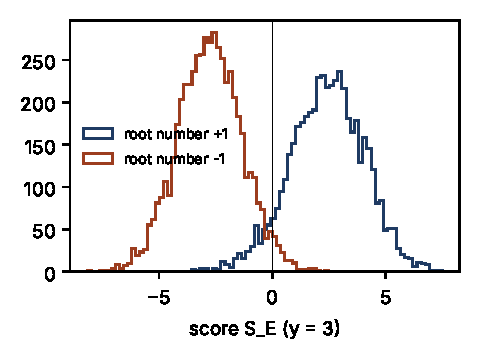
\includegraphics[width=0.55\textwidth]{figs/murm_score.pdf}
\caption{Histograms of the murmuration score $S_E$ with $y=3$ for the held out classes of root number $+1$ and $-1$ with $5000\le N<10000$.}\label{fig:05bscore}
\end{figure}

The transfer column is the most telling. A density learned on conductors $5000$ to $10000$ and applied, through $y=p/N$ alone, to conductors $2500$ to $5000$ classifies the smaller curves slightly better than the held out curves of its own window. Scale invariance is therefore not only visible in Figure~\ref{fig:05bdensity}; it is predictive.

\section{Murmurations, one level density and Thorin measures}\label{sec:05bthorin}

\subsection{The edge of the support}

Chapter~\ref{ch:06} described the low lying zeros of families of $L$ functions through their one level densities. For the family of weight two newforms of level $N$, normalised so that the zeros near the centre are spaced at mean distance one, Iwaniec, Luo and Sarnak \cite{ils2000} proved that the subfamilies of root number $+1$ and $-1$ have the one level densities of the orthogonal groups $\mathrm{SO}(\text{even})$ and $\mathrm{SO}(\text{odd})$, for test functions $\phi$ whose Fourier transform is supported in $(-2,2)$, assuming the generalized Riemann hypothesis. Including the central zero forced by the root number $-1$, the Fourier transforms of these two densities coincide on $(-1,1)$ and differ by $1$ for $|u|>1$ \cite{katzsarnak1999}. In the explicit formula the variable $u$ is $\log p/\log N$ up to constants, so the edge $|u|=1$ is the scale $p\approx N$. The root number is invisible to the low lying zeros unless the test function reaches primes of the size of the conductor.

This is where murmurations live. As $X\to\infty$ the whole window $0<y\le3$ of Figure~\ref{fig:05bdensity} collapses, on the logarithmic scale of $u$, to the single point $u=1$. The random matrix limit records what happens there as a step; murmurations are the arithmetic structure of the step at finite conductor, resolved on the linear scale $y=p/N$. We do not know a statement that makes this precise, and we pose one as Open Problem~\ref{op:05bedge}.

\subsection{Thorin form}

By Theorem~\ref{thm:10bmain}, under the generalized Riemann hypothesis for $L(s,E)$, the reciprocal of the completion of Chapter~\ref{ch:10b}, with the central zero of order $r_E$ removed, is the Laplace transform of a generalized gamma convolution whose Thorin measure is
\[
U_E=\sum_k\delta_{\gamma_k^2},
\]
the sum running over the ordinates $\gamma_k\ne0$ of the noncentral zeros $\frac12+i\gamma_k$, with multiplicity. Rescale each atom by the mean spacing, $t\mapsto t\,(\log N_E/2\pi)^2$, and call the result $\tilde U_E$. The one level density of the family is then the average of the measures $\tilde U_E$ read through $t\mapsto\sqrt t$, and the root number weighted average
\[
\Delta_X=\frac{1}{\#\mathcal{F}_X}\sum_{E\in\mathcal{F}_X}\varepsilon_E\,\tilde U_E
\]
is a signed measure that, in the random matrix limit and read in the symmetric variable $x=\pm\sqrt t$, has the density $2\sin(2\pi x)/(2\pi x)$: the difference of the two orthogonal densities with their central zeros removed. Its Fourier transform in $x$ is the indicator of $(-1,1)$, with its jump at the edge. Murmurations should therefore be visible in the Thorin measures as a correction to $\Delta_X$ whose Fourier transform is concentrated at $|u|=1$. Since the Thorin framework removes the central zeros, it isolates exactly the part of the family that the root number moves.

\section{Ramanujan, Mordell and the Hecke operators}\label{sec:05bram}

The tools of this chapter are older than the Langlands programme, and they begin with two Cambridge papers. In 1916 Ramanujan \cite{ramanujan1916} studied the coefficients of
\[
\Delta(z)=q\prod_{n\ge1}(1-q^n)^{24}=\sum_{n\ge1}\tau(n)q^n,\qquad q=e^{2\pi iz},
\]
and conjectured from his tables three properties: $\tau(mn)=\tau(m)\tau(n)$ for coprime $m,n$; the recursion $\tau(p^{j+1})=\tau(p)\tau(p^j)-p^{11}\tau(p^{j-1})$; and the bound $|\tau(p)|\le2p^{11/2}$. The first two say that $L(s,\Delta)=\sum\tau(n)n^{-s}$ has the Euler product $\prod_p(1-\tau(p)p^{-s}+p^{11-2s})^{-1}$, and the third says that the roots of each local factor have absolute value $p^{11/2}$, so that $x_p=\tau(p)/p^{11/2}$ lies in $[-2,2]$ like the normalised traces of an elliptic curve. A year later Mordell \cite{mordell1917} proved the first two. His proof averages $\Delta$ over the $p+1$ cosets that define what is now the Hecke operator $T_p$, and observes that the result is again a cusp form of weight twelve and level one, hence a multiple of $\Delta$; the multiple is $\tau(p)$. Hecke \cite{hecke1937} turned the argument into a theory twenty years later, and the bound waited for Deligne \cite{deligne1974}. Ramanujan's $x_p$ are one of the data sets of Chapter~\ref{ch:05}, where their empirical law is compared with the Sato Tate law.

Every step of Section~\ref{sec:05bdef} is a descendant of Mordell's averaging. The murmuration average over a family is a trace of $T_p$, possibly composed with $W_N$, and the trace is computed by the Eichler Selberg formula \cite{eichler1973,selberg1956}, which expresses it through Hurwitz class numbers. For level one it has a particularly clean form \cite{zagier1977}: for $k\ge4$ even and $p$ prime,
\begin{equation}\label{eq:05besf}
\operatorname{tr}\bigl(T_p\mid S_k(1)\bigr)=-\frac12\sum_{t\in\Z,\ t^2<4p}P_k(t,p)\,H(4p-t^2)-1,\qquad P_k(t,p)=\frac{\rho^{k-1}-\bar\rho^{\,k-1}}{\rho-\bar\rho},
\end{equation}
where $\rho,\bar\rho$ are the roots of $X^2-tX+p$ and $H$ is the Hurwitz class number. For $k=12$ the space $S_{12}(1)$ is spanned by $\Delta$, and \eqref{eq:05besf} gives $\tau(2)=-24$, $\tau(3)=252$ and $\tau(5)=4830$, as we checked numerically.

\subsection{Ramanujan's family in the weight aspect}

Ramanujan's $\Delta$ is the first member of a family: the Hecke eigenforms of level one and weight $k$, of which there are $\dim S_k(1)\approx k/12$. All of them share the root number $\varepsilon_k=i^k=(-1)^{k/2}$, since $\Lambda(s,f)=(2\pi)^{-s}\Gamma(s)L(s,f)$ satisfies $\Lambda(s,f)=(-1)^{k/2}\Lambda(k-s,f)$. So in this family the root number is a function of the weight, and the murmuration average is simply the trace \eqref{eq:05besf} divided by the dimension, with sign $\varepsilon_k$. The results of Bober, Booker, Lee and Lowry Duda \cite{bbllp2023} are at the scale $y=p/k^2$. Writing $P_k(t,p)=p^{(k-2)/2}\sin((k-1)\theta_t)/\sin\theta_t$ with $t=2\sqrt p\cos\theta_t$, the reason is visible in \eqref{eq:05besf}: the phase $(k-1)\theta_t$ moves by about $k/(2\sqrt p)=1/(2\sqrt y)$ from one $t$ to the next.

We evaluated \eqref{eq:05besf} for every even weight $100\le k<400$ ($150$ weights, $3{,}025$ eigenforms) and every prime $p\le3.2\times10^5$, with the Hurwitz class numbers from PARI/GP, and averaged $\varepsilon_k\lambda_f(p)$, where $\lambda_f(p)=a_f(p)/p^{(k-1)/2}\in[-2,2]$, over the forms and over the primes in bins of $y=p/k^2$. Two observations, both empirical:

\begin{enumerate}
\item The average decays like $1/k$: its root mean square over $0<y\le2$, in bins of width $0.025$, falls from $0.0130$ for $100\le k<150$ to $0.0048$ for $280\le k<400$, a ratio of $2.7$, against a ratio of mean weights of $2.7$. After multiplication by $k$ the densities of the windows $100\le k<200$ and $200\le k<400$ agree, with correlation $0.81$ over $40$ bins of width $0.05$, and closely for $y<0.5$ (Figure~\ref{fig:05bweight}).
\item The density is concentrated: in bins of width $0.01$ its largest values occur near $y=0.025$ and $y=0.235$, and it changes sign sharply at $y=\frac14$, the point at which, in the heuristic above, the phase step $1/(2\sqrt y)$ equals one radian.
\end{enumerate}

Our normalisation, scaling by $k$ and binning are ours, not those of \cite{bbllp2023}, and the comparison of Figure~\ref{fig:05bweight} with their limiting density is left as Computational Problem~\ref{cp:05bweight}. Compared with the weight two family of Section~\ref{sec:05bdata}, the weight aspect has a single root number per weight and no ranks, so it isolates the trace formula mechanism from the rank bias of Section~\ref{sec:05brank}.

\begin{figure}[ht]
\centering
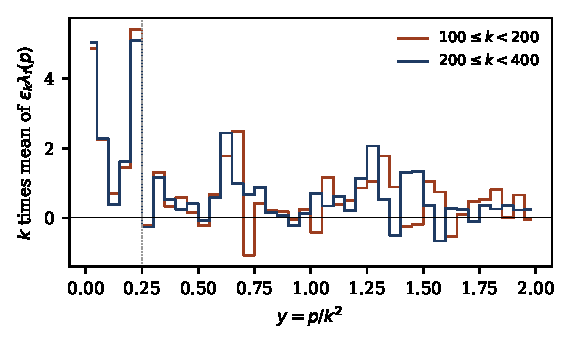
\includegraphics[width=0.66\textwidth]{figs/murm_weight.pdf}
\caption{Murmurations in Ramanujan's family: $k$ times the average of $\varepsilon_k\lambda_f(p)$ over the level one eigenforms of weight $k$, in bins of $y=p/k^2$ of width $0.05$, computed from the trace formula \eqref{eq:05besf}, for $100\le k<200$ and $200\le k<400$. The dotted line marks $y=\frac14$.}\label{fig:05bweight}
\end{figure}

\subsection{Mordell's theorem and the rank}

Mordell's second contribution is the reason the word rank means anything. In 1922 he proved that the group $E(\Q)$ of rational points of an elliptic curve is finitely generated \cite{mordell1922}, so that $E(\Q)\cong\Z^{r}\oplus T$ with $T$ finite. The murmurations of Section~\ref{sec:05bdata} separate curves by $\varepsilon_E=(-1)^{r_E^{\mathrm{an}}}$, the parity of the analytic rank, not by Mordell's $r$. The two agree when the analytic rank is $0$ or $1$, by Gross and Zagier \cite{grosszagier1986} and Kolyvagin \cite{kolyvagin1988}, which covers $19{,}347$ of the $20{,}728$ classes of the window $[5000,10000)$; for the remaining classes of analytic rank $2$ and $3$ the equality with $r$ is a computation recorded in Cremona's tables \cite{cremonaecdata}, an instance of the parity conjecture that is not known in general. So the statement ``murmurations see the parity of the Mordell Weil rank'' rests, beyond rank one, on Birch and Swinnerton Dyer.

Mordell's name is also attached to the equation $y^2=x^3+k$. These curves have complex multiplication by $\Z[\frac{1+\sqrt{-3}}2]$, so $a_p=0$ for every $p\equiv2\bmod3$, and the Sato Tate law of Chapter~\ref{ch:04} is replaced by the law of the CM group, half an atom at $0$. Their root numbers are computable from $k$ by local formulas. Whether this family shows murmurations, and how the atom at $0$ and the CM structure change the density, is Computational Problem~\ref{cp:05bmordell}. The Mordell conjecture, proved by Faltings \cite{faltings1983}, concerns curves of genus at least two, which have finitely many rational points and no rank to correlate with; it plays no role here.

\section{Notes}

The original paper of He, Lee, Oliver and Pozdnyakov \cite{hlop2022} contains the plots that started the subject, for curves in the LMFDB of conductor up to about $10^4$ and for ranks $0$, $1$ and $2$. Sarnak's letter \cite{sarnakletter2023} gave the trace formula explanation. Zubrilina's proof \cite{zubrilina2023} uses the Eichler Selberg trace formula in the form for $T_n\circ W_N$; the computation of such traces goes back to Yamauchi \cite{yamauchi1973}. The weight aspect \cite{bbllp2023} and Dirichlet characters \cite{lop2023} followed in 2023, and elliptic curves ordered by height in 2025 \cite{sawinsutherland2025}. The murmuration score, the model of Definition~\ref{def:05bmodel} and the calibration in Table~\ref{tab:05bclass} are ours. Cremona's tables \cite{cremonaecdata} are complete for the conductors used here, and the scripts \texttt{murm.py}, \texttt{analysis.py} and \texttt{figs\_ch.py} in the directory \texttt{murm} of the repository reproduce every number in this chapter. Mordell's 1917 proof \cite{mordell1917} of Ramanujan's multiplicativity conjectures \cite{ramanujan1916} is the first appearance of the Hecke operators on which every proof of murmurations rests; the level one trace formula in the form \eqref{eq:05besf} is in Zagier \cite{zagier1977}, and the weight aspect computation of Section~\ref{sec:05bram} uses only that formula and PARI/GP.

\section{Exercises}

\begin{enumerate}
\item Show that for a weight two newform $f$ of level $N$ with trivial character the functional equation $\Lambda(s,f)=\varepsilon_f\Lambda(2-s,f)$, with $\Lambda(s,f)=N^{s/2}(2\pi)^{-s}\Gamma(s)L(s,f)$, holds with $\varepsilon_f=-w_f$, where $w_f$ is the eigenvalue of the Atkin Lehner involution. Deduce that $\sum_f\varepsilon_fa_f(n)=-\operatorname{tr}(T_n\circ W_N)$.
\item Verify the identity $\varepsilon_E=(-1)^{r_E}$ on the four curves $11a1$, $37a1$, $389a1$ and $5077a1$ of Chapter~\ref{ch:05}, computing the root numbers with \texttt{ellrootno} in PARI/GP.
\item Let $S$ be the score of Definition~\ref{def:05bmodel} with weights $m_p$ and suppose the $x_p$ are independent given $\varepsilon$ with means $\varepsilon m_p$ and variances $\sigma_p^2$. Show that the weights $w_p$ that maximise the signal to noise ratio $\E[\varepsilon S_w]/\operatorname{sd}(\varepsilon S_w)$ of $S_w=\sum_pw_px_p$ are $w_p\propto m_p/\sigma_p^2$. For the Sato Tate law, $\sigma_p^2=1$; why is this not the right variance at the bad primes?
\item In the setting of Proposition~\ref{prop:05bclass}(3), suppose instead that $\varepsilon=+1$ has prior probability $\theta$. Find the Bayes rule and its error probability, and evaluate them for $\theta=0.478$, the frequency of root number $+1$ in the window $[5000,10000)$, and $V=2.58$.
\item (Rank mixtures.) Suppose that given $\varepsilon=+1$ the rank is $0$ with probability $q$ and $2$ with probability $1-q$, and that given the rank $r$ the $x_p$ are independent normal with means $m_p+b_r$ and variance $1$, where $b_0=\beta$ and $b_2=-3\beta$ for a constant $\beta>0$, and similarly given $\varepsilon=-1$ the rank is $1$ with means $-m_p-\beta$. Write down the posterior probability of $\varepsilon=+1$ and show that the error of the rule $\operatorname{sign}S$ for rank $2$ curves tends to $1$ when $\beta\,\#P$ is large compared with $V$.
\item Using the prime number theorem, show that the number of pairs $(E,p)$ with $E\in\mathcal{F}_X$ and $y\le p/N_E<y+h$ is asymptotic to $\#\mathcal{F}_X\cdot hX\,c_y/\log X$ for a constant $c_y$ that you should identify, under the assumption that the conductors in $\mathcal{F}_X$ are spread over $[X,2X)$ with a continuous density. Deduce the order of the standard error of $D_X(y)$.
\item (Mordell's argument.) Let $f\in S_{12}(1)$ and define $T_pf(z)=p^{11}f(pz)+p^{-1}\sum_{j=0}^{p-1}f\bigl(\frac{z+j}p\bigr)$. Show that $T_pf\in S_{12}(1)$, compute its $q$ expansion, and deduce from $\dim S_{12}(1)=1$ that $\tau(pn)=\tau(p)\tau(n)-p^{11}\tau(n/p)$, with $\tau(n/p)=0$ when $p\nmid n$.
\item Verify \eqref{eq:05besf} for $k=12$ and $p=2,3$ by hand, using $H(3)=\frac13$, $H(4)=\frac12$, $H(7)=1$, $H(8)=1$, $H(11)=1$, $H(12)=\frac43$.
\end{enumerate}

\section{Open problems}

\begin{problem}[Conductor ordering]\label{op:05bcond}
Prove that the murmuration density $D_X(y)$ of Definition~\ref{def:05bmurm} converges as $X\to\infty$, for elliptic curves over $\Q$ ordered by conductor, one curve per isogeny class, and identify the limit. Is it the density $M$ of Theorem~\ref{thm:05bzub} for all weight two newforms, suitably normalised, or does the restriction to rational coefficients change it?
\end{problem}

\begin{problem}[Posterior concentration]\label{op:05bpost}
In the murmuration model with the rank bias added (Exercise 5), find the rate at which the Bayes error for the root number tends to zero, or to a positive limit, as the cutoff $y$ and the conductor grow together. Is $\int_{y_0}^y D(t)^2\,dt/t$ the governing quantity, as Lemma~\ref{lem:05bsignal} suggests, and why are the observed scores more concentrated than the model predicts?
\end{problem}

\begin{problem}[The edge]\label{op:05bedge}
Let $\Delta_X$ be the root number weighted average of the rescaled Thorin measures of Section~\ref{sec:05bthorin}. Assuming the generalized Riemann hypothesis for the family, show that the Fourier transform of $\Delta_X$, after subtraction of its random matrix limit, converges in a window of width of order $1/\log X$ around $|u|=1$, and that the limit is determined by the murmuration density. We do not know whether this is the right formulation; the question is whether the Thorin measures see murmurations at all.
\end{problem}

\section{Open computational problems}

\begin{compproblem}[Murmurations to conductor $500{,}000$]\label{cp:05bscale}
Objective: extend Figure~\ref{fig:05bdensity} to all isogeny classes of conductor below $500{,}000$ in Cremona's tables, in dyadic windows. Route: \texttt{ellan} in PARI/GP up to $3N$ for each class, or Harvey's average polynomial time method for all $p\le1.5\cdot10^6$ at once \cite{harvey2014}. Deliverable: $D_X(y)$ with standard errors in each window, a test of convergence in $X$, and a comparison with the density of Theorem~\ref{thm:05bzub} and with the prime conductor prediction of Sawin and Sutherland \cite{sawinsutherland2025}. Why it matters: it is the evidence on which Open Problem~\ref{op:05bcond} rests.
\end{compproblem}

\begin{compproblem}[Kinks at $y=t^2/4$]
Objective: decide whether $D_X(y)$ shows changes of slope at $y=\frac14$, $1$ and $\frac94$, where the trace formula heuristic of Section~\ref{sec:05bdef} has new terms entering. Route: the data of Computational Problem~\ref{cp:05bscale} with bins of width $0.005$ near these points, and local polynomial fits on each side. Deliverable: estimated jumps in the derivative with confidence intervals.
\end{compproblem}

\begin{compproblem}[Root numbers in higher degree]
Objective: test whether murmuration scores recover root numbers for genus two curves, whose $L$ functions have degree four. Route: the genus two curves of the LMFDB \cite{lmfdb} with their analytic ranks, traces $a_p$ from \texttt{hyperellcharpoly} in PARI/GP, and the classifier of Section~\ref{sec:05bbayes} with the abelian conductor in place of $N$. Deliverable: the murmuration density for genus two curves, if it exists, the accuracy table analogous to Table~\ref{tab:05bclass}, and the dependence on the Sato Tate group in the sense of Chapter~\ref{ch:12}.
\end{compproblem}

\begin{compproblem}[The weight aspect]\label{cp:05bweight}
Objective: compare Figure~\ref{fig:05bweight} with the limiting density of Bober, Booker, Lee and Lowry Duda \cite{bbllp2023}, and decide whether the decay like $1/k$ observed in Section~\ref{sec:05bram} is the correct normalisation. Route: \eqref{eq:05besf} with Hurwitz class numbers tabulated once, for all even $k\le2000$ and $p\le2k^2$; smoothing over $k$. Deliverable: the density in the variable $y=p/k^2$ with error bands, and the locations of its singular points, in particular at $y=\frac14$.
\end{compproblem}

\begin{compproblem}[Mordell curves]\label{cp:05bmordell}
Objective: test for murmurations in the family $y^2=x^3+k$, $1\le|k|\le K$, sixth power free. Route: conductors, root numbers and $a_p$ from \texttt{ellglobalred}, \texttt{ellrootno} and \texttt{ellan} in PARI/GP for $K$ up to $10^6$; bins of $y=p/N$ with the primes $p\equiv2\bmod3$, where $a_p=0$, excluded and included separately. Deliverable: the analogue of Figure~\ref{fig:05bdensity} for this family and a comparison with the full family of Section~\ref{sec:05bdata}. Why it matters: it shows whether murmurations survive in a thin family with complex multiplication, where the Sato Tate group is not $\SU(2)$.
\end{compproblem}
